\chapter{Experimental Setup}
\label{chap:exp}
The accelerators are utilized to recreate the high energy environment rich in new physics like the hot early universe. In this thesis, Large Hadron Collider (LHC) is used for this purpose, and the ATLAS detector (A Toroidal LHC ApparatuS) is taken to probe the potential signatures of new physics. 
\section{Large Hadron Collider\cite{LHC}}
LHC is a circular collider with a diameter of 27~km for hadrons (it could be either protons or lead ions) hosted by CERN at the border of France and Switzerland in the depth varied between 50m to 175m. It accelerates protons (lead ions) to the speed of Lorentz Factor of 10540 (32) and smashes them together to recreate the ``hot'' environment right after the big bang which corresponds to 6.5~TeV (2.5~TeV) energy. However, before a proton reaches the targeted energy, it has a long way to go.
\\
\\{\bf Ionization}
\\
\\At the beginning, hydrogen is released from a tank and ionized into the state of proton-electron plasma. It then experiences the electric field to separate electrons as well as protons like Fig. \ref{Fig:ionization}. The protons are then taken out and sent into the LINAC2, a linear accelerator. After reaching the energy of $450MeV$, the protons are fed into circular accelerators in the order of the PSB, PS and SPS to further increase the energy until they reach 450$~GeV$ (Fig. \ref{Fig:boost}). By this stage, the protons are ready to be injected into the LHC.
\begin{figure}[!h]                
	\includegraphics[width=0.8\textwidth]{Chapter2/ionization.png}
	\centering
	\begin{center}
		\caption{The hydrogen plasma is separated into electrons (red) and protons (blue), and the protons are injected into LINAC2. This image is taken from \cite{Ionization}.}
		\label{Fig:ionization}            
	\end{center}
\end{figure}
\\
\begin{figure}[!h]                
	\includegraphics[width=0.95\textwidth]{Chapter2/pre-acceleration.jpg}
	\centering
	\begin{center}
		\caption{Before the LHC, protons go through several boosting facilities. This material is taken from \cite{Mobs:2197559}}
		\label{Fig:boost}            
	\end{center}
\end{figure}
{\bf Magnets}
\\
\\While accelerating the protons, they  would repel each other due to the same electric charge they are carrying, so the quadrupole magnets are implemented in LHC to focus them by the effect of magnetic lens. In addition to the quadrupole magnets, the other magnet system in LHC is the superconducting dipole magnets working to bend the protons to keep them staying in the circular pipe of the LHC. The dipole system was upgraded between 2012 and 2015 to provide a 8.3~T magnetic field to bend the proton beam at an energy of 6.5~TeV.
\\
\\{\bf Radiofrequency Cavity\cite{Radiofrequency:1997424}}  
\\
\\The ``radiofrequency cavity'' (RF cavity) is in charge of the acceleration. Protons would experience electric field when going through RF cavities which are installed in the LHC like beads along a string. The field is induced by an alternating current of a frequency of $400~MHz$ and resonates as a standing wave in the cavity. This wave decelerates faster protons and accelerates slower ones, which makes the protons squeeze into bunches as demonstrated in Fig. \ref{Fig:bunch}., until they reach the targeted energy. When the beams are kept in the same speed, they are called ``stable beams'' and ready for the collision. 
\begin{figure}[!h]                
	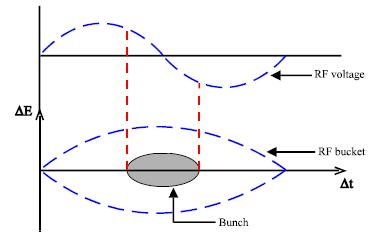
\includegraphics[width=0.3\textwidth]{Chapter2/bunch.png}
	\centering
	\begin{center}
		\caption{The protons are formed into a bunch in the EM wave. This image is taken from \cite{Baird:1017689}}
		\label{Fig:bunch}            
	\end{center}
\end{figure}
\noindent
\\
\\Each LHC beam could have up to 3564 bunches with $\mathcal{O}^{12}$ protons in each bunch for a spacing of 25~ns, but not all of them are filled. For the LHC 2018 operation, the ``filling scheme''  has around 1000-2500 bunches filled, while the remaining ones are left empty (filling scheme most of time is constrained due to technical issues). A series of continuous bunches is called a ``bunch train''. This scheme would then be used to configure the trigger and data acquisition system for the active window of detector operation.
\\  
\\{\bf Collision}
\\
\\The LHC has two beams going in opposite directions with the same configuration (bunch structure, luminosity and energy), and the two beams cross at locations where four detectors are sited: ALICE\cite{alicetdr}, ATLAS\cite{atlastdr}, CMS\cite{cmstdr}, and LHCb\cite{lhcbtdr}. Before stable beams, the two beams pass each other where they are supposed to cross. When both of the beams are ready, the two beams are slightly shifted to target on each other for the collisions .  The crossing angle between the two beams plays an important role in detector performance. It should not be too big, or it would have an impact on physical object reconstruction (see section. \ref{sec:obj rec}) which assumed a zero crossing angle. However, it also should not be too small, or the two beams would interfere with each other. The crossing angle is kept optimized during LHC operation even when the detectors are taking data for physics.
\\
\\When collisions happen, the two crossed bunches usually have more than one pair of interacting protons. In physics, only the most energetic one gets the attention for study, while the other ones are the background contribution called "pile-up events". For ATLAS 2018 operation, the pile-up events could number up to 70 per bunch crossing, and it is now a major challenge of analyses to suppress this type of background.
\\
\\The collisions are then taken as ``instant luminosity'' for the measurement on the amount of data:
\begin{equation}
\mathcal{L}_{inst} = \frac{N}{t\times S^{eff}}
\end{equation}
with N as the number of collisions and $S^{eff}$ as the effect area of the LHC beams for the collisions \footnote{$S^{eff}=4\times\pi\times(1.6\times 10^{-5})^2[m^2]$ for the LHC configuration.}. Then, the total collected data with time is presented as:
\begin{equation}
\mathcal{L} = \int \mathcal{L}_{inst}dt
\end{equation} 
\section{ATLAS Detector}
The ATLAS detector (A Toroidal LHC ApparatuS) \cite{Airapetian:391176} is designed as a general purpose detector\footnote{The other general purpose detector hosted by LHC is Compact Muon Solenoid (CMS). The discovery of any new physics shall be verified by both the ATLAS and CMS collaborations} aiming for most high energy physics physics topics in the energy scale LHC provides like SM precision measurement and searches for new physics.

The ATLAS detector is in a cylinder shape with dimensions of 44m in length and 25m in diameter. Its inner structure is like an onion with multiple layers from the inner most tracking system to the outer part of muon spectrometer functioning to capture different physical objects which will be explained in the following. In the purpose of measuring the particle mass and charge, ATLAS also has two magnetic systems (a solenoid and a toroid) located outside inner tracking system and muon spectrometer. The diagram of the whole ATLAS detector is shown in Fig. \ref{Fig:ATLAS} with the two minimum bias trigger scintillators (MBTS) at both ends.

\begin{figure}[!h]                
	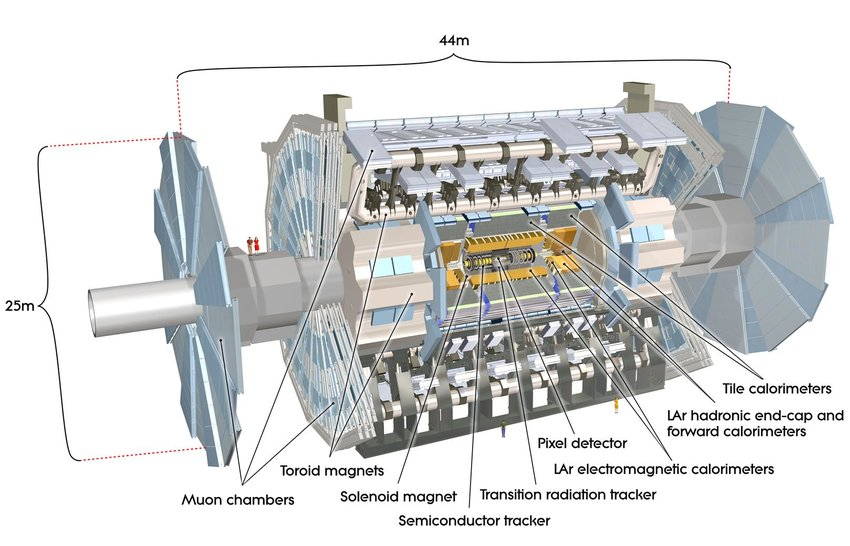
\includegraphics[width=0.8\textwidth]{Chapter2/ATLAS.jpg}
	\centering
	\begin{center}
		\caption{The diagram of the ATLAS detector taken from \cite{Collaboration_2008}}
		\label{Fig:ATLAS}            
	\end{center}
\end{figure}

To define the object positions inside this massive and complicated giant, the coordinate is applied as shown in Fig. \ref{Fig:coordinate}. The x-axis is defined pointing to the centre of the LHC, while the z-axis is the cylinder axle toward the direction of solenoid magnetic field. Then, the y-axis could be found with the right-hand rule. However, this Cartesian coordinate is not convenient in a cylinder, so, instead, the spherical system ($\theta$:angle related to z-axis, $\phi$:angle related to x-axis) is adopted in terms of physics. To keep the parameters as Lorentz invariance, $\theta$ is interpreted into pseudorapidity, $\eta$:
\begin{equation}
\eta = -\ln{\tan{\frac{\theta}{2}}}
\end{equation}
\begin{figure}[!h]                
	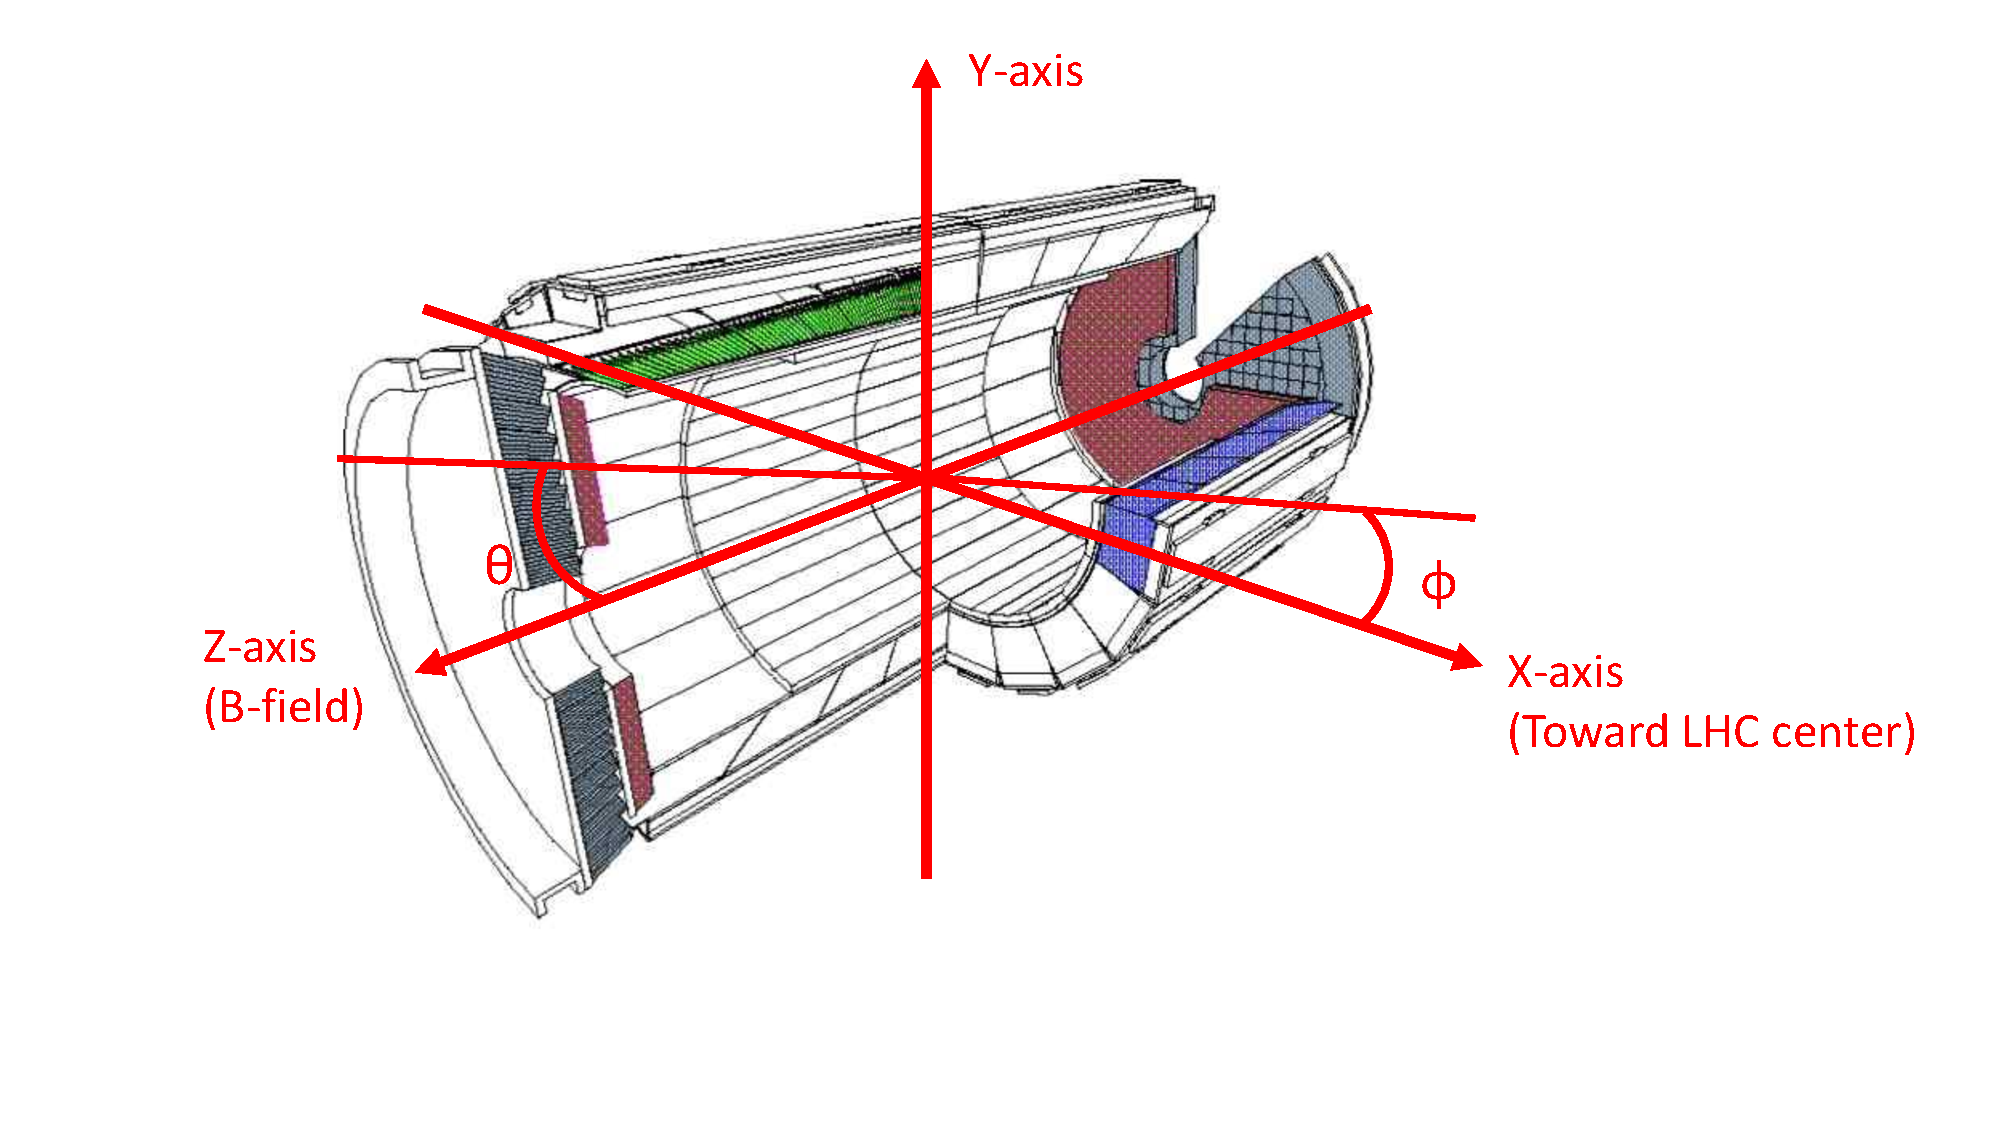
\includegraphics[width=0.95\textwidth]{Chapter2/coordinate}
	\centering
	\begin{center}
		\caption{The coordinate system used in the ATLAS detector}
		\label{Fig:coordinate}            
	\end{center}
\end{figure}
With this definition, the variation of $\eta$ is different from $\theta$, which can be seen in Fig. \ref{Fig:pseudorapidity}. This quantity is important, because the distance between two particles in the detector is defined as:
\begin{equation}
\Delta R= \sqrt{\Delta \eta^{2}+\Delta \phi^{2}}
\end{equation}
For the same $\Delta R$, the separation would be actually larger in the high $\eta$ region especially at $|\eta|>3.2$ (``endcap'' and ``forward'' regions).  
\begin{figure}[!h]                
	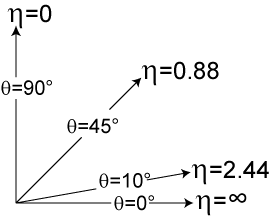
\includegraphics[width=0.4\textwidth]{Chapter2/pseudorapidity.png}
	\centering
	\begin{center}
		\caption{The Psedorapidity varied with $\theta$ from \cite{pseudorapidity_wiki}}
		\label{Fig:pseudorapidity}            
	\end{center}
\end{figure}

\subsection{Inner Detector (ID) \cite{CERN-LHCC-97-016}}
%remember to mention MBTS
The design of a general detector usually consists of two types of system: ``trackers'' and ``calorimeters''. The tracker is used to record the particle trajectories inside the detector with the lowest disturbance on its energy, while calorimeters trap the particles to measure its total energy sum, $E$. 
\\
\\The ATLAS Inner detector is designed as a ``tracker'', so it is used to take the tracks of particles from the collisions. It stands at the inner most part of the detector and spans from 3cm to 108cm in radius with several layers from three subsystems which are pixel, semiconductor tracker (SCT) and transition radiation tracker (TRT) as shown in Fig. \ref{Fig:ID}. 

\begin{figure}[!h]                
	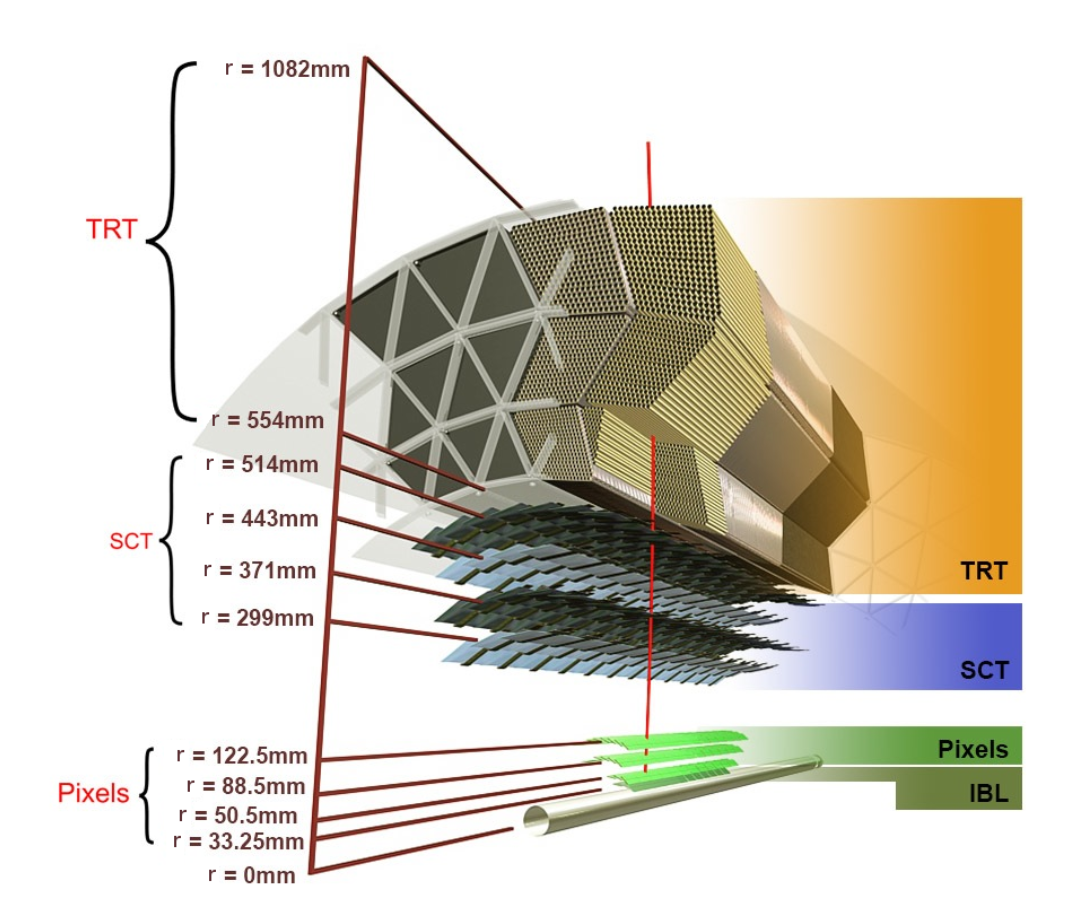
\includegraphics[width=0.7\textwidth]{Chapter2/ID.png}
	\centering
	\begin{center}
		\caption{The diagram for the ATLAS inner detector from \cite{PERF-2015-08}}
		\label{Fig:ID}            
	\end{center}
\end{figure}

Each layer has cells of well-defined granularity. When particles are passing through the inner detector, they leave ``a hit'' per cell on each layer. The tracks are then defined as the link through hits on each layer which are curved lines due to the existence of magnetic field from solenoid, so the curvature of a track could be taken to evaluate the particle momentum and charge. After all tracks are reconstructed, the vertexes are then defined as where the tracks cross. The resolution of transverse momentum, $p_{T}$\footnote{In ATLAS, the activity on transverse plane (i.e. x-y plan) has most of physics interest, because the transverse momentum sum is supposed to be 0, but the case for longitudinal direction isn't}, depends on the particle $p_{T}$ and $\eta$, and it can be presented as:
\begin{equation}
\sigma_{p_{T}} = \sqrt{a^{2}p_{T}^{4}+b^{2}p_{T}^{2}}
\end{equation}
with a and b, the coefficients, depending on track quality and $\eta$. From MC simulation for the track with lease seven hits (a track crossing all layers from pixel and SCT) within $0.25<|\eta|<0.5$, a and b are estimated to be 0.00034 $~GeV^{-1}$ and $0.0015$ respectively.
\\
\\{\bf Pixel\cite{Collaboration:2285585}}
\\
\\The pixel detector is the innermost system of ATLAS, and it has the structure of three concentric barrels enclosed by three disks at each end, so all the particles coming out from the collision must pass through all the layers (giving three hits). It provides the best position resolution in the ATLAS detector with a granularity of $50~\mu m\times 400~\mu m$  for each cell in the $r\Delta \phi \times z$ plane with the coverage of $|\eta|<2.5$ which is used to define the barrel region which has a spatial resolution of $14~\mu m\times 115~\mu m$
\\
\\In 2014, a new layer of pixel detector called insertable b-layer (IBL) \cite{Miucci_2014} was installed at $3.3~cm$ to the beam pipe in addition to the original three layers. Its design is aiming to assist with measurements of short-live particles (like the b quarks whose lifetime is $~10^{-12}~s$), so it has an even better granularity of $50~\mu m\times 250~\mu m$ with extended coverage to $|\eta|<3$. The improved granularity also helps to reduce the uncertainty on impact parameter of collisions.
\\
\\{\bf Semiconductor Tracker}
\\
\\Outside the pixel detector is the semiconductor tracker with three layers in its barrel and nine disks at each end. The sensors are double sided, so when a particle passes through four layers, it leaves totally eight hits in the SCT which form four spacepoints. Different from the pixel detector which has one sensor on each module, the SCT modules have two strip sensors with the width of $80~\mu m$ which cross at  an angle of $40~mrad$ giving a spatial resolution of $17~\mu m \times 580~\mu m$ in the $r\Delta \phi \times \Delta z$ plane. 
\\
\\{\bf Transition Radiation Tracker}
\\
\\The last part of the inner detector is the TRT detector. It doesn't have a multiple layer structure as the pixel or SCT detectors but just a single thick layer stacked of straw drift tubes. Each straw has the diameter of 4~mm (with the drift time correction, the spatial resolution from each measurement is $130~\mu m$) and is filled with the gas mixture of $Xe$, $CO_{2}$ and $O_{2}$. The gas mixture is used to optimize the absorption of transition radiation. (Due to the gas leaking problem found in the ATLAS operation from 2009 to 2012 \cite{Mindur:2139567}, part of the gas was replaced by cheaper $Ar$-based gas.) When a charge particle passes through the gas, the emitted photon (transition radiation) induces a ``charge avalanche''. This detector allows to the distinguish between electrons and charged pions (because light particles emit more transition radiation).
\\
\\{\bf Magnets}
\\
\\ The ATLAS detector has two superconducting magnet systems different from the CMS experiment with only one solenoid magnet. The inner one is the solenoid magnet located between the TRT detector and the calorimeter, while the toroid magnet is situated in the muon spectrometer system. The advantage of this design is to have the light material (solenoid) inside the detector for transparency, and the toroid still provides the magnetic field to further improve the resolution of momentum measurement\cite{magnets}.  
\\
\\The solenoid magnet is with a diameter of $2.56~m$ and length of $5.8~m$.  The magnetic field inside the solenoid is almost uniform of 2~T along the z-axis as shown in Fig.~\ref{Fig:bfield} to give the momentum and charge measurement in the inner detector. 
\begin{figure}[!h]                
	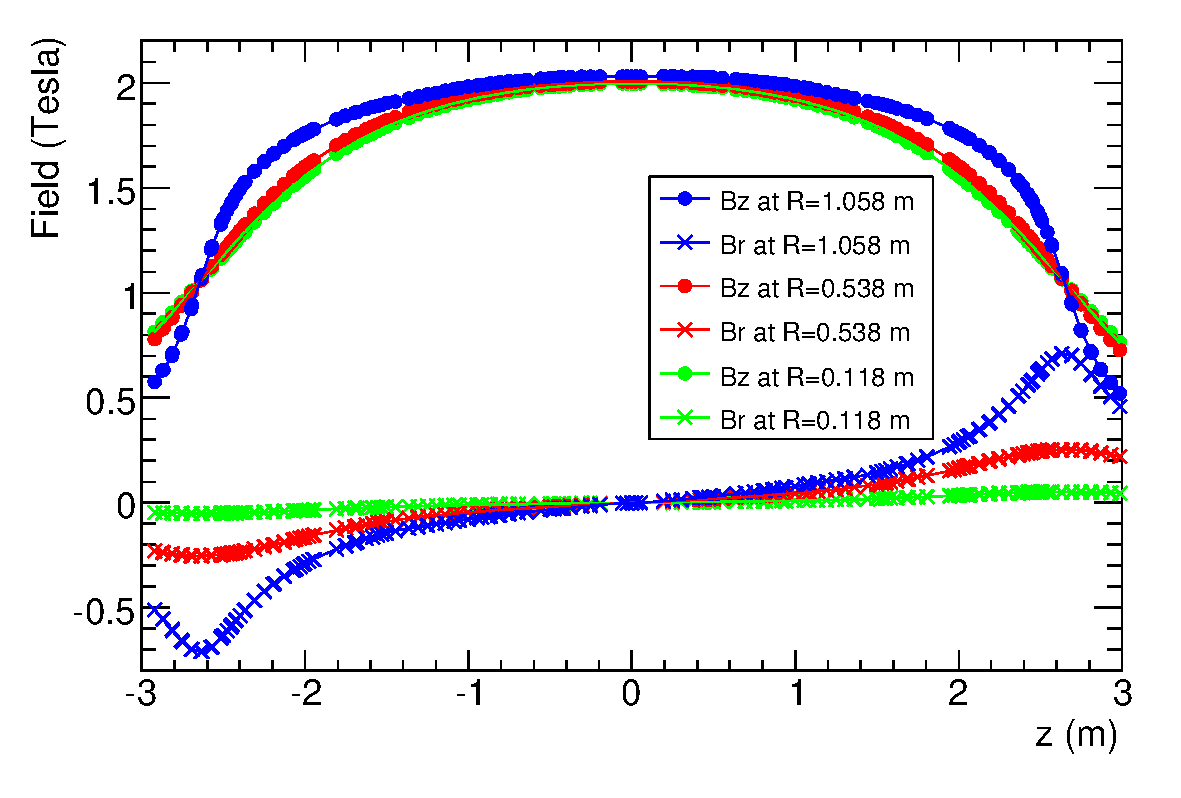
\includegraphics[width=0.6\textwidth]{Chapter2/bfield}
	\centering
	\begin{center}
		\caption{The magnetic field inside the solenoid taken from \cite{Aleksa_2008}}
		\label{Fig:bfield}            
	\end{center}
\end{figure}
\\
\\The toroid magent is composed of the barrel and endcap toroids, and both of them have eight coils providing the magnetic field of 4~T in the muon spectrometer. The toroid magnet has the advantage that the particle trajectories in the transverse plane are always perpendicular to the magnetic field, so the momentum measurement is simplified. The toroid magnet is for the measurement of muon momentum in the muon spectrometer. 
\subsection{Calorimeter}
Outside the inner detector is the calorimeter, an energy sampling system. In the ATLAS analyses, there is the need to distinguish the fundamental particles with their energy, so two systems of calorimeters are applied to trap particles with different mass: the electromagnetic calorimeter (ECAL) for electrons and photons as well as the hadronic calorimeter (HCAL) for the hadronic particles. Both ECAL and HCAL have the coverage up to $|\eta|<4.9$. For the range of $|\eta|<2.5$ in the barrel region, two types of calorimeter, the liquid argon (LAr) and tile detectors, are used for the ECAL and HCAL, while in the endcap and forward regions is only the LAr detector. To fit into the cylinder shape of the ATLAS detector, the calorimeters are accordion-shaped from the cross section side. The full diagram of the calorimeter system is presented in Fig. \ref{Fig:calorimeter}. 
\begin{figure}[!h]                %
	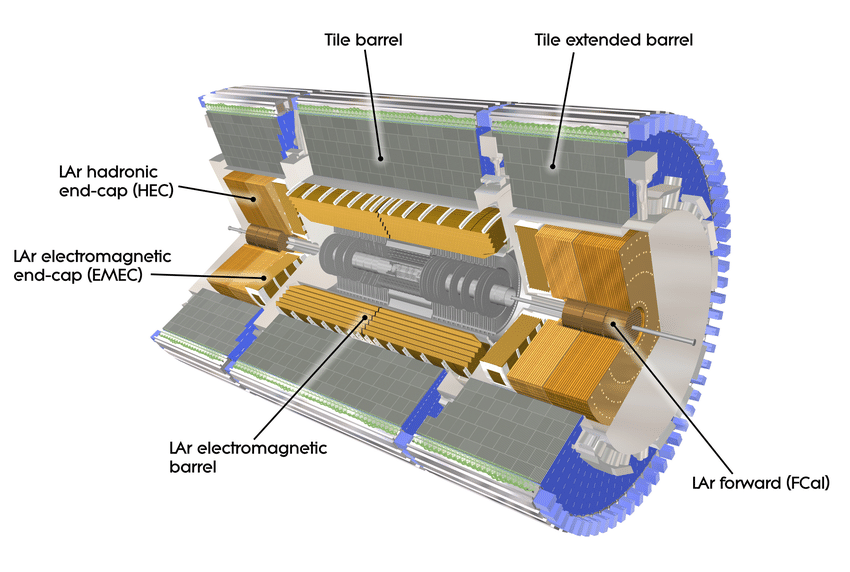
\includegraphics[width=0.85\textwidth]{Chapter2/calorimeter}
	\centering
	\begin{center}
		\caption{The calorimeter system of the ATLAS detector from \cite{Aad:2008zzm}}
		\label{Fig:calorimeter}            
	\end{center}
\end{figure}
The energy resolution for the calorimeter could be presented as:
\begin{equation}
\sigma (E)=\sqrt{a^{2}+b^{2}E+c^{2}E^{2}}
\end{equation}
where a, b, and c are the coefficients. The first term is due to the electronic noise (constant), and the second term is from the shower development of the Poisson fluctuation for the number of shower particles, while the third terms is for the calorimeter non-uniformities (linear to the true shower energy). From the test beam data, the coefficients for the ECAL are $0.4~GeV$, $0.1~\sqrt{GeV}$ and $0.0017$ for a, b, and c. In terms of the HCAL, the resolution is a bit worse with $1.6~GeV$, $0.52~\sqrt{GeV}$ and $0.03$. The degraded resolution is due to the intrinsic property of the measurement on hadronic objects which have the energy contribution from neutrinos or binding energy between hadrons. 
\\
\\{\bf Electromagnetic Calorimeter}
\\
\\In ATLAS, the ECAL is made up of the LAr detector\cite{ATLAS:1996ab} each module of which has one absorber and one electrode, and liquid argon is the medium between them. When a particle hits the absorber, it induces the shower, and the shower electrons ionize liquid argon atoms. All the electrons from the interactions would then be collected by the electrodes. The measured current is used to estimate the energy of the incoming particle. The process could be seen in Fig. \ref{Fig:larshower}.\\
\begin{figure}[!h]                
	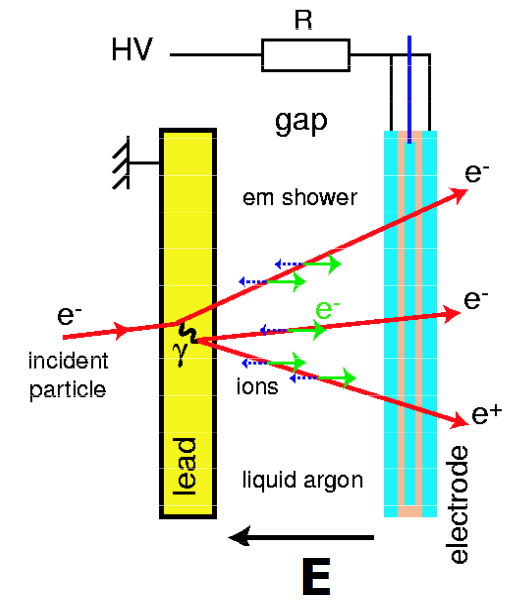
\includegraphics[width=0.35\textwidth]{Chapter2/LArshower}
	\centering
	\begin{center}
		\caption{The interaction between an electron and the LAr calorimeter taken from \cite{LArwork}}
		\label{Fig:larshower}            
	\end{center}
\end{figure}
\\The barrel LAr detector has three sampling layers with different depth and granularity. An extra presampler (layer 0) was added for $|\eta|<1.8$ which has no absorber but only a thin LAr sampler to recognize photons from $\pi^{0}$ decays. The best granularity is at the strip layer (layer 1) for $0.0031\times ~0.1$ ($\Delta \eta \times \Delta \phi$) \footnote{the granularity for $\Delta \phi$ is a approximation, as it has to complete a circle of an irrational number.}, while the last layer is coarse for $0.05 \times ~0.025$ in terms of $\Delta \eta \times \Delta \phi$. For the energy absorption, the depth is what matters most. The full depth of the three sampling layers could correspond to $\sim$22 lead radiation lengths ($X_{0}$) or 2 nuclear interaction length ($2\lambda$).\footnote{the radiation length is defined by the electron energy loss, while the nuclear interaction length is defined by the hadronic object energy loss.} When the ECAL is extended to the region of $2.5<|\eta|<3.2$, only the last two layers would remain, but they still have $18X_{0}$ in total.
\\
\\{\bf Hadronic Calorimeter}
\\
\\Behind the LAr detector is the three-layer tile detector covering $|\eta|<1.7$ with a crack\footnote{The crack is for the supporting structure and output cables} at $1.37<|\eta|<1.52$. It operates in the similar way to the LAr detector, but the absorber material is scintillator. Each sensor of this system is coarser as compared to LAr ones with $0.1 \times ~0.1$ ($\Delta \eta \times \Delta \phi$) for the first two layer and $0.1 \times 0.2$ at the third layer. With the need for the absorption of hadronic objects, it has $8 \lambda$ in the depth for all three layers.
\\
\\In the endcap region ($1.7<|\eta|<3.1$), another type of LAr detector with copper absorber is used as the HCAL. It contains four layers which have the same granularity for $0.1 \times 0.1$ ($\Delta \eta \times \Delta \phi$) in the region, $1.7<|\eta|<2.5$, and $0.2 \times 0.2$ in $2.5<|\eta|<3.1$
\\
\\{\bf Forward Calorimeter \cite{Artamonov_2008}}
\\
\\In contract to the inner detector, the calorimeter should capture as many particles as possible, so the missing energy carried by invisible particles could be estimated by energy conservation within the detector. Therefore, a forward detector is installed at $3.1<|\eta|<4.9$, and it has the best rapidity coverage among the ATLAS subsystems. 
\\
\\The type of detector used here is the third type of LAr detector with tungsten absorber. It has three layers with the first one for ECAL and the last two for HCAL with the same depth of $10\lambda$ (ECAL+HCAL).  
\subsection{Muon Spectrometer\cite{MS_all}}
The outermost detector is the muon spectrometer (MS). Because of their large mass and lack of strong interactions, only muons could travel through the calorimeter and leave signatures here. The muon spectrometer is composed of four types of detectors: thin gap chamber (TGC), resistive plate chamber (RPC), monitored drift tubes (MDT), and cathode strip chamber (CSC) with the toroid magnet system.  
\\
\\In this subsystem, the MDT and CSC are the two detectors providing the tracking measurement with a three-layer structure. In the coverage of $|\eta|<2.0$, all the three layers are composed of the MDT detector, while the innermost layer is replaced by the CSC detector in the extent of $2.0<|\eta|<2.7$ for the effectiveness of high particle density environment. The overall tracking measurement has the spatial resolution of $35 \mu m$
\\
\\However, the precise tracking measurement of the MDT and CSC comes with the cost of a poor temporal resolution, so the RPC ($|\eta|<1.05$) and TGC (($1.05<|\eta|<2.7$)) are interspersed in tracking layers with the time resolution of $25~ns$ (with the consideration of uncertainty from cosmic muons). With the fast response, they are part of the ATLAS hardware trigger system. The overall detector performance is summarised in Tab. \ref{Tab:ms}.

\begin{table}[h]
	\caption{Muon Spectrometer Subdetector Performance}
	\renewcommand{\arraystretch}{1.3}
	\centering
	\begin{tabular}{l | c | c | c | c | c }
		\hline
		\hline
		{\bf Type}     &{\bf Function} &{\bf coverage}    &{\bf z/R resolution}  &{\bf $r \Delta \phi$ resolution}&{\bf time resolution}\\
		\hline
		MDT            &tracking       &$|\eta|<2.7$      &$35~\mu m$(z)          &N/A                             &N/A            \\
		\hline
		CSC            &tracking       &$2.0<|\eta|<2.7$  &$40~\mu m$(R)          &$5~mm$                           &$7~ns$          \\
		\hline
		RPC            &trigger        &$|\eta|<1.05$     &$10~mm$(z)             &$10~mm$                          &$1.5~ns$         \\
		\hline
		TGC            &trigger        &$1.05<|\eta|<2.7$ &$2-6~mm$(R)            &$3-7~mm$                         &$4~ns$           \\
		\hline
	\end{tabular}
	\label{Tab:ms}
\end{table}

\subsection{Trigger System}
The LHC has the collision rate at $~40MHz$, which leads to the data rate over $60~TB$ per second. However, most of the events have no physical interest, because they are just the products of low energy hadronic interactions. Therefore, the trigger system is developed to select events which are going to the storage.
\\
\\For data-taking, the ATLAS trigger system has a two-level structure: the hardware-based L1 trigger (L1) and the software-based high level trigger (HLT). The L1 system is based on the front-end electronics with the logic of selection written by FGPA. Its feature is to make a fast reconstruction of physical objects with a degraded resolution, and it delivers the events at the rate of $100~kHz$ ($100k$ events per second). As the detector signatures from the calorimeter and MS are irrelevant to each other, they have their independent L1 trigger systems: L1Calo and L1MU. After the physical objects objects are reconstructed in the two systems, they are then sent to the L1Topo system for the estimation on the topological relation between them. The final trigger decision would eventually be made at the central trigger processor (CTP) by whether a event contains the objects with energy or topological parameters fulfilling the defined criteria. Afterwards, those objects are further processed with a more complicated reconstruction algorithm to give the HLT trigger decision, and the output event rate is reduced to $\sim 1~kHz$. The full trigger system is shown in Fig. \ref{Fig:trigger}.

\begin{figure}[!h]                
	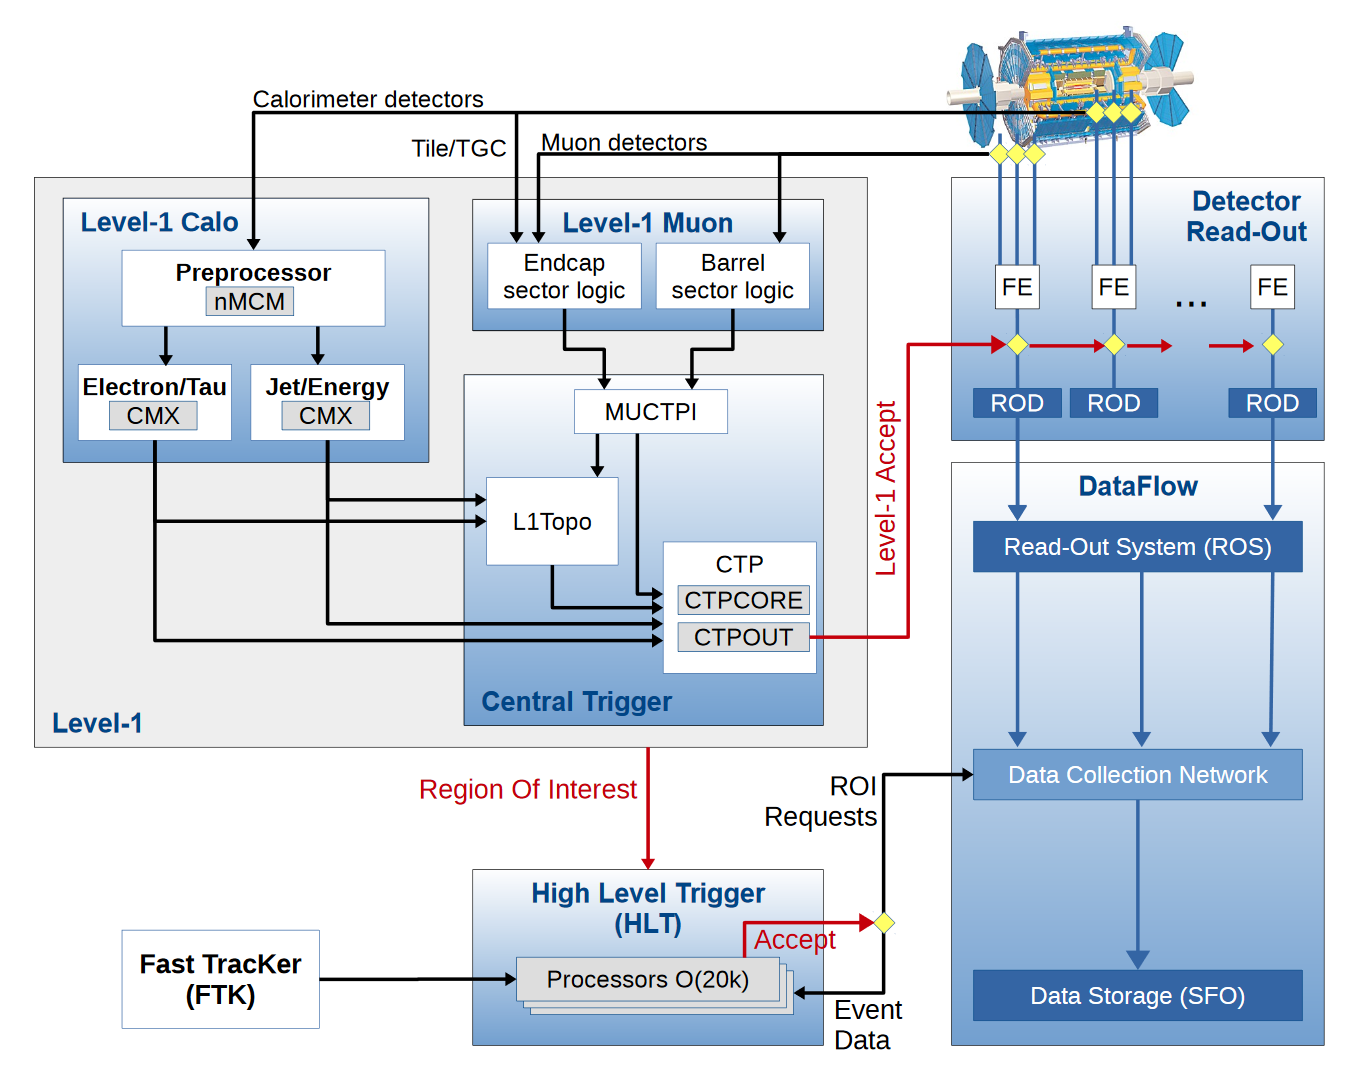
\includegraphics[width=0.8\textwidth]{Chapter2/Trigger.png}
	\centering
	\begin{center}
		\caption{The ATLAS trigger system from \cite{trigger_str}}
		\label{Fig:trigger}            
	\end{center}
\end{figure}
\noindent
\\{\bf L1Calo}
\\
\\When the detector signatures are received from the calorimeter, they are firstly sent to the readout buffer and the L1Calo sysetm. The first component in the L1Calo electronic system is the preprocessor where the signatures are processed into trigger towers with degraded granularity and sent to the processors for physical object reconstruction. Electrons, photons and taus are reconstructed with the trigger tower of $0.1 \times 0.1 (\Delta \eta \times \Delta \phi)$ in the cluster processor (CP), while hadronic objects and missing transverse energy ($E_{T}^{missing}$)\footnote{As the protons only have the longitudinal momentum, the transverse direction momentum should be conserved after collisions} are processed in jet energy processor (JEP) with a coarser granularity of $0.2\times 0.2$.
\\
\\{\bf L1MU}
\\
\\The L1MU system is taking the data from the RPC and CSC which have great time resolution as fast as $1.5~\mu s$ but with a poor spatial resolution. It receives signatures from the MS barrel and endcaps where they are processed respectively. To further suppress the rate contributed by fake muons, the L1 muons are reconstructed with consistent hits from the TGC at the endcap ($1.05<|\eta|<2.7$). 
\\
\\{\bf HLT}
\\
\\When the trigger decision was made to accept an event, the regions of interest (ROI) with the original detector granularity are passed to the HLT. The HLT is runs on a CPU farm where the more complicated algorithms are deployed to reconstruct the physical objects. Due to the finer granularity and longer latency, it provides better precision on both energy and spatial resolution. When the events fulfil the HLT criteria, they are then sent to storage. 
\\
\\{\bf ATLAS Trigger Menu}
\\
\\An ATLAS trigger is generally a trigger chain composed of L1 and HLT items. When an HLT trigger is fired, there is always a corresponding L1 trigger decision. For example, HLT electron trigger shall only be passed when a L1 electron trigger is also fired:
\begin{equation}
L1\_e24 \rightarrow HLT\_e26\_lhtight\_nod0\_ivarloose
\end{equation}
where the numbers are the trigger thresholds in the unit of $GeV$, while the $lhtight$ and $ivarloose$ are to define the electron quality with the calorimeter activities in the surrounding region of this electron (see more details in Sec. \ref{sec:obj rec}) . The threshold of triggers might not be kept the same during the operation at periods. Because the LHC keeps pushing its performance on instantaneous luminosity, the energy contribution from pile-up events enhances the trigger rate above the allowed bandwidth for data storage. To make better suppression on the trigger rate, the thresholds are therefore raised during some operation periods. 
\\
\\The defined triggers would then be made into ``streams'' where the events are categorized for different purposes. Physics analyses shall use the triggers contained in the ``$physics\_main$'' stream, and there are also the dedicated streams composed of ``prescaled'' triggers for hardware calibrations. Those calibration triggers usually have lower thresholds in contract with the ones in $physics\_main$. A random sampling is applied to only pick a fraction of events passing those triggers, which makes them unsuitable for physics analysis. The total allowed output rate from all streams is $5~kHz$ with $1~kHz$ for $physics\_main$. 

\subsection{Run 2 Operation Overview}
For the ATLAS operation from 2015 to 2018 which is called Run 2 (with respect to Run 1 from 2009 to 2013), the average data recording efficiency is around $95\%$ with respect to LHC delivery efficiency. From the measurement with the Lminosity  Cherenkov  Integrating  Detector (LUCID, one of the forward detectors of the ATLAS)\cite{Bruschi:2025000, ATLAS:2019pzw}, the integrated luminosity is $\sim~36fb^{-1}$ for 2015 and 2016, $\sim46~fb^{-1}$ for 2017 and $\sim63~fb^{-1}$ for 2018 which gives the total data of $140 fb^{-1}$. The performance from 2011 to 2018 is summarized in Fig. \ref{Fig:recefficiency}
\begin{figure}[!h]                
	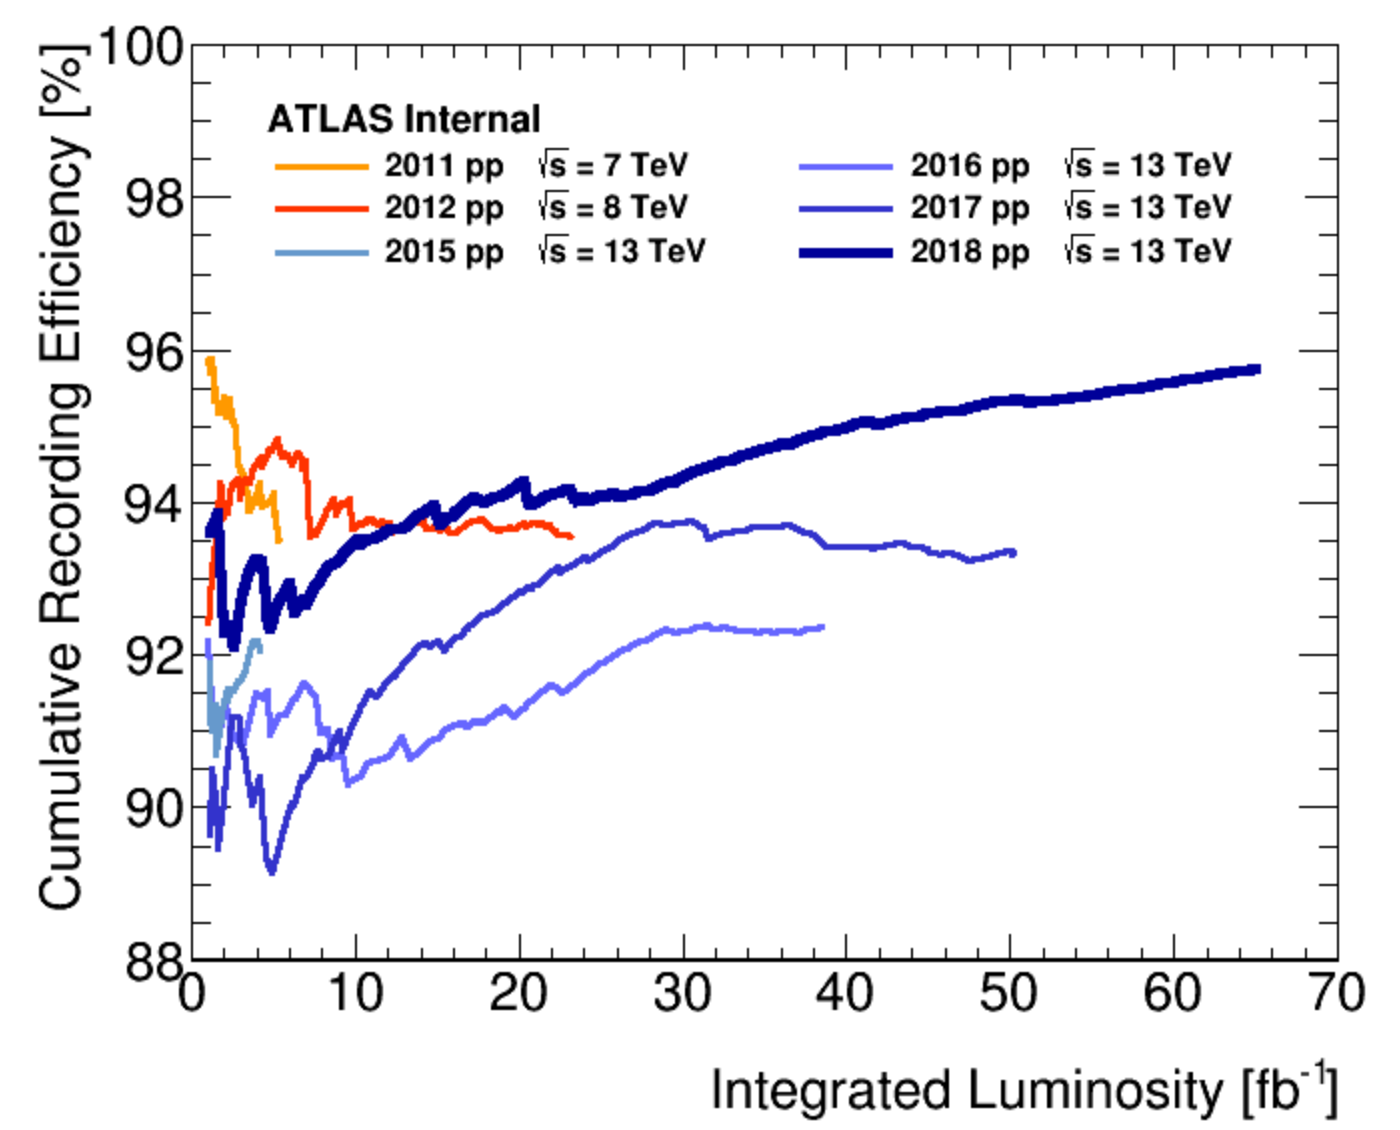
\includegraphics[width=0.6\textwidth]{Chapter2/recefficiency.png}
	\centering
	\begin{center}
		\caption{The ATLAS recording efficiency and luminosity \cite{Pontecorvo:2638061}}
		\label{Fig:recefficiency}            
	\end{center}
\end{figure}
\section{Object Reconstruction}
\label{sec:obj rec}
When the events are passed into the permanent storage, they are still in the format of raw data which contains only the information of hits (the spacepoints from the inner detector and muon spectrometer) and calorimeter energy towers (the energy deposited in the calorimeter cells). They need to go though the full reconstruction (offline reconstruction) to be interpreted into the objects with physical meanings as the SM particles like electrons or muons. The reconstruction will be based on the principles of interactions between detectors and particles: 
\\
\\1) Only charged particles leave tracks in the inner detector
\\
\\2) The charged particles shall deposit energy in the ECAL, and the light ones are stopped here.
\\
\\3) All the particles except for muons are supposed to be stopped in or before the HCAL.
\\
\\4) Only muons could reach the muon spectrometer. 
\\
\\After the reconstruction of all subjects, a further correction on energy scale (the peak of the energy pulse shape) is applied on both data and simulation samples to take in  the effect of energy loss from the radiation, the contamination from other objects, or the detector effect (like dark current, hot noise, or material inhomogeneities). The final procedure is to remove the overlapped objects by the priority defined by the analyses. 
\\
\\{\bf Primary Vertex $\&$ Tracks \cite{Aaboud:2017all}}
\\
\\A pattern recognition is performed in the SCT to find the helical trajectories with at least 3 spacepoints and $p_{T}>500MeV$ which are taken as the track seeds. A Kalman Filter algorithm is then performed to extend the track seeds to the pixel layers. To resolve the reconstruction ambiguity, a tracking score system is taken to reject the shared spacepoints or fake tracks. When a track is reconstructed with more hits and less ``holes'' (missing hits in some layers), it is given a higher score. The final tracks shall all have at least seven hits (three spacepoints from SCT and four hits from pixel). To complete the track reconstruction, the projection route from the outermost SCT spacepoint of a track passes through TRT, and the drift tubes within $10mm$ from the route are integrated into the track. Afterwards, one addition track reconstruction (outside-in) from TRT is performed to recover the tracks from the late decay or photon conversion. The unused TRT segments are then rematched to the SCT and pixel hit remanent.   
\\
\\The crossing points of tracks near the LHC pipelines are then assumed to be where the interactions happen, which are called ``vertices''. The vertex associated with the highest $p_{T}^2$ sum is then defined as the primary vertex. All the reconstructed objects should origin from the primary vertex which is verified by $d_{0}$ and $d_z$, the distances between the object and the primary vertex in the x-y plane and the z-axis, or they are taken as ``minimum bias'' background.  
\\
\\{\bf Electrons}
\\
\\Electrons are charged light particles, so they leave tracks in the inner detector and energy clusters in the ECAL. The two types of signature are combined and testified to reconstruct electrons.
\\
\\The first stage of the reconstruction is to build the energy cluster as an electron seed \cite{ATLAS-CONF-2016-024,ATL-LARG-PUB-2008-002}. A window of $3 \times 5$ ECAL layer-2 cells (corresponding to $0.075 \times 0.125$ in $\Delta \eta \times \Delta \phi$) is used to scans through ECAL layer-2 to find the electron seeds. If the transverse energy sum ($E_{T}$) inside the window is above $2.5GeV$, the cells inside this window are selected, and the electron position is defined as the energy weighted $\eta$ and $\phi$ (barycentre) of this window. Then, this window is extended along the $R$-direction to sum over the energy in other layers with the adjusted window size (detailed in ~\cite{}). The cells taken in the cluster are then removed to avoid the duplication into other electrons. With the estimation from $Z\to ee$ simulation sample, this algorithm has the electron reconstruction efficiency of $95\%$ ($>99\%$) for $E_{T}\sim7GeV$ ($E_{T}>15GeV$).
\\
\\The reconstruction of tracks associated to electrons is performed independently from the mentioned reconstruction . A track seed of $p_{T}>1GeV$ is firstly reconstructed with three spacepoints from the SCT layers . Then, based on the pion hypothesis (pion energy loss pattern in the ID materials), it is verified by whether this track seed can be extended to pixel with four hits and matched to a calorimeter cluster. If it fails, the electron hypothesis is applied for the same verification. The hits from both hypotheses are then fitted using ``ATLAS Global $\chi^{2}$ Track Fitter''\cite{Cornelissen:2008zza} into tracks, and the tracks failing the pion track hypothesis are then tested again with electron hypothesis. The tracks passing the electron hypothesis are then taken as potential electron tracks. This algorithm is also integrated in the standard track reconstruction with the least interference.
\\
\\The track and cluster are then associated with a loose $\Delta R$ matching which considers the electron bremsstrahlung and the number of hits in the inner detector. The matched track-cluster pairs are then refitted with optimised ``Gaussian Sum Filter'' (GSF) \cite{ATLAS-CONF-2012-047} to take non-linear bremsstrahlung into account. 
\\
\\To have further separation between signal-like and background-like electrons, the electron identification is then performed on $Z \rightarrow ee$ (signal) and dijet (background) MC samples. It is a multi-variable analysis (MVA) based on the likelihood discriminant defined as:
\\
\begin{equation}
d_{\mathcal{L}}=\frac{\mathcal{L}_{S}}{\mathcal{L}_{S}+\mathcal{L}_{B}}    
\quad \text{ and } \quad
\mathcal{L}_{S(B)}(\vec{x})=\prod_{i = 1}^{n}P^{i}_{S(b)}(x^{i})
\end{equation}
where $P^{i}_{S(b)}(x^{i})$ is the probability density function for a specific input variable $x^{i}$, and $\vec{x}$ is the vector formed by them in the likelihood phase space of all input variables (all the input variables could be found in \cite{}). Three working points are therefore defined by $d_{\mathcal{L}}$: $Tight$, $Medium$ and $Loose$\footnote{$Tight$ selected electrons are the subset of $Medium$, and $Medium$ is the subset of $Loose$}. The signal efficiency from this selection process is as a function of electron $E_{T}$, and the plateau of efficiency could be reached at $E_{T}~70GeV$ for $~97\%$ ($~95\%$) [$91\%$] on $Loose$ ($Medium$) [$Tight$] working point. 
\\
\\In addition to the reconstruction quality, the electrons are also required to be ``isolated'' from all the other tracker and calorimeter signatures, because of the concern that the nearby detector activities might affect the electron measurement. The isolation is defined in two ways: 
\begin{itemize}
	\item the calorimeter isolation ($Iso^{E_{T}}$): it is defined as the cluster $E_{T}$ sum within a cone with $R=0.2(0.3)$ centred at the reconstructed electron inside which a central cluster subset in a rectangle of $0.125 \times 0.175$ ($\Delta \eta \times \Delta \phi$) is subtracted.
	\item the track isolation ($Iso^{p_{T}}$): it is defined as the $p_{T}$ sum of tracks from primary vertext within a cone of $R=min(0.2(0.3), 10GeV/E^{e}_{T})$ centred at the electron but without the electron associated tracks.  
\end{itemize}
The isolation discriminant is then applied as $Iso^{E_{T}}/E_{T}$ or $Iso^{p_T}/p_{T}$. The recommendation working points on the discriminant are given as a function of $E^{e}_{T}$ or fixed cut which are summarised with the muon isolation working points in Tab. \ref{Tab:iso}. 
\\
\\{\bf Muons \cite{Herde:2059849}}
\\
\\Muons are heavy enough to travel through the calorimeter and reach the MS, but the reconstruction is mainly based on the tracks in the inner detector and the MS. 
\\
\\The MS track segments are firstly built from the hits within each MS module, but the reconstruction coordinates are different in each subsystem: the MDT reconstruction is on the coordinate of the toroid magnetic bending plane, while the RPC and TCG have the coordinate orthogonal to it, and the CSC is only using the detector $\eta$-$\phi$ coordinate. A loose criteria is applied in the segment building algorithm to verify the compatibility to a full track. Then, the segments in the middle layer of the MS are taken as the track seed and extended to the inner and outer layers. If two segments could be fitted with enough hits by matching from their relative position and angle, they are integrated into the same track. The exception is in the transition region between the barrel and endcap, and a standalone and good-quality segment could be kept as a single track.  
\\
\\An overlap removal is afterwards applied to remove the shared hits in the tracks with poor fitting quality, but they could still be kept only if the fitting criterion is fulfilled. Two tracks could share maximally two hits in the inner two layers and have no same hit in the outer layer for the concern of close-by muons. 
\\
\\The hits along the tracks are then taken into the global $\chi^{2}$ fitting. The hits with great deviation from the fitted MS trajectory are removed, and the fit is applied again to derive the new track. If there are hits not included in the track but within the allowed deviation from the track, they are also taken into the track, and the fitting is repeated. 
\\
\\The final MS tracks are taken as the seed to match to the inner detector tracks to reconstruct the combined muons. A further global fitting is conducted to extrapolate the muons with the flexibility to add in or remove the MS hits to improve the fitting quality with the ID tracks. The primary algorithm in the fitting is performed outside-in from the MS to the inner detector, and a complementary algorithm of inside-out is also applied to guarantee the robustness of the reconstruction. For the muons outside of the inner detector coverage ($2.5<|\eta|<2.7$), they can be reconstructed from only MS tracks, but the criteria are more stringent. 
\\
\\Similar to electrons, muons also have the identification procedure with three parameters: $q/p$ significance (the ratio of charge and momentum measured in the ID and MS over the quadrature sum of their uncertainty), $\rho'$ (the ratio of momentum difference between the ID and MS measurements over the combined measurement) and the normalised combined track fit, $\chi^2$. The working points for the muons identification have the definition individually as below:
\begin{itemize}
	\item $Medium$ muons: they are defined within the range of $0.1<|\eta|<2.5$ with at least two layers of $\geq 3$ hits. If it is within the range, $0.1<|\eta|$, it is allowed to have hits in only one layer, but there shall be no hole in the MS track reconstruction. As the muons go beyond the coverage of the inner detector (i.e. $2.5<|\eta|<2.7$), they shall have the MS tracks reconstructed from all three layers. An extra requirement of $q/g$ significance above seven is also applied on this muon quality. 
	\item $Loose$ muons: those muons are defined with the most loose requirement. They are generally $Medium$ muons, but the selection is loosen for the range of $|\eta|<0.1$ due to the missing coverage of the MS (where a gap is present for the service of the ID and calorimeter). When an ID track is found within this range and matched to a calorimeter cluster which is identified as a deposit by ``minimum-ionization'' particles, they are also accepted as loose muons to recover the reconstruction efficiency. 
	\item $Tight$ muons: all of them must have the tracks reconstructed from two layers in the MS (either MDT or CSC) with $Medium$ muon hit selection. To enhance the purity of muons, a further requirement on the ID to MS track fitting is also added into the selection for $\chi^2<8$. An addition two-dimension cut on $q/g$ significance and $\rho'$ is also applied to improve the background rejection for muons with $p_{T}<20GeV$.
\end{itemize}
For the muon isolation, the definition is similar to the electron ones, but they have different working points. The recommended working points for electrons and muons are shown in tab. \ref{Tab:iso}.

\begin{table}[h]
	\caption{Electron/Muon Isolation Working Points}
	\renewcommand{\arraystretch}{1.5}
	\centering
	\begin{adjustbox}{center}
		\begin{tabular}{|c | c | c | c | c |}
			\hline
			\hline
			{\bf Working Point} &{\bf Object} &{\bf Calo Iso}                   &{\bf Track Iso}  &{Combined Iso} \\
			\hline
			LoseeTrackOnly      &all leptons  &-                                      &$99\%$                 &$99\%$               \\
			\hline
			Loose               &all leptons  &\multicolumn{2}{|c|}{$99\%$}                                   &$99\%$               \\
			\hline
			Gradient            &all leptons  &\multicolumn{2}{|c|}{$\epsilon=(0.1143*p_{T}[GeV]+92.14)\%$}   & \shortstack{\footnotesize{$\epsilon(25GeV)=90\%$} \\  \footnotesize{$\epsilon(60GeV)=99\%$}}\\       
			\hline
			GradientLoose       &all leptons  &\multicolumn{2}{|c|}{$\epsilon=(0.057*p_{T}[GeV]+95.57)\%$}   & \shortstack{\footnotesize{$\epsilon(25GeV)=95\%$} \\  \footnotesize{$\epsilon(60GeV)=99\%$}}\\
			\hline
			FixedCutTight       &Electrons  &\footnotesize{topoetcone20/pT<0.06}                 &\footnotesize{ptvarcone20/pT<0.06}  &-               \\
			\hline
			FixedCutTight       &Muons  &\footnotesize{topoetcone20/pT<0.06}                 &\footnotesize{ptvarcone30/pT<0.06}  &-               \\
			\hline
			\footnotesize{FixedCutTightTrackOnly}      &Electrons     &-                 &\footnotesize{ptvarcone20/pT<0.06}  &-               \\
			\hline
			\footnotesize{FixedCutTightTrackOnly}      &Muons      &-                 & \footnotesize{ptvarcone30/pT<0.06}  &-               \\
			\hline
			FixedCutLoose        &Electrons  & \footnotesize{topoetcone20/pT < 0.2} & \footnotesize{ptvarcone20/pT < 0.15}  & - \\
			\hline
			FixedCutLoose        &Muons  & \footnotesize{topoetcone20/pT < 0.3} & \footnotesize{ptvarcone30/pT < 0.15}  & - \\
			\hline
			\footnotesize{FixedCutHighPtCaloOnly} & Electrons &  \footnotesize{topoetcone20} < 3.5 GeV & - &-\\
			\hline
			\footnotesize{FixedCutHighPtTrackOnly} & Muons &  - &  \footnotesize{ptcone20} < 1.25 GeV  &-\\
			\hline
		\end{tabular}
	\end{adjustbox}
	\label{Tab:iso}
\end{table}
\noindent
{\bf Jets}
\\
\\When quarks or gluons are travelling in the space, they went through the process called ``fragmentation'' or ``hadronization'' for ``color-confinement'' of QCD. This leads to the multiplication of quarks, gluons (i.e. partons) or even leptons and photons, and they eventually form the bound states as hadrons leaving complicated signatures in the detector. One quark from a collision might leave more than one hundred tracks in the inner detector and several clusters in the calorimeter, and jets are defined as the ensemble of those signatures. To properly collect those tracks and calorimeter clusters into the same jets, the reconstruction algorithm is designed to ensure the infrared safety and collinear safety. The infrared safety means that 
the soft radiation from hadronic objects in a jet would not change the jet width or orientation, while the collinear safety indicates that the nearby particles with higher $p_{T}$ in the collinear direction of the splitted parton would not affect the jet reconstruction. To achieve both of the two requirements, the jet reconstruction algorithm\cite{Atkin:2015msa} employs the following two parameters for the jet definition: 
\begin{equation}
d_{ij}=min((p_{t}^{i})^{a},(p_{t}^{j})^{a})\times \frac{R_{ij}^{2}}{R}
\quad \text{ with } \quad
d_{iB}=(p_{t}^{i})^{a}
\end{equation}
where $p_{t}^{i}$ and $p_{t}^{j}$ are $p_{T}$ of $i$th and $j$th entities which could be calorimeter clusters (a patch of energetic cells in the calorimeter), tracks, or the truth particles from the simulation, $R_{ij}$ is the distance between them, and R is the parameter to customize the algorithm for performance (i.e. cone size), while $a$ corresponds to three algorithms which are sensitive to different jet properties. $a=-2$ is for $anti-k_{t}$ algorithm, and it has the advantage for better stability of jet structure during reconstruction with high sensitivity to hard objects and ignorance for the jet substructure as well as pile-up events. $a=0$ and $a=-2$ are used for Cambridge-Aachen algorithm and $k_{t}$ algorithm respectively which are more sensitive to jet substructure but with high dependence on pile-up events and soft objects. When $d_{ij}<d_{iB}$, the $i^{th}$ and $j^{th}$ objects are merged into the same cluster with the position defined as their barycentre. If no new pair could be found meeting this condition, the cluster is then defined as a jet. To make further 
\\
\\For the jets in the ATLAS experiment, $anti-k_{t}$ algorithm is preferred with $R=0.4$ and $R=1.0$ with the inputs objects. $R=1.0$ is for the scenario that two jets are close to each other, and $R=0.4$ could not have the separation power to distinguish each of them. The input entities for jet reconstruction is the ECAL topo clusters in the range of $|\eta|<4.9$, the calorimeter coverage, with energy $2\sigma$ above the quadrature sum of pile-up events and electronic noise, while the seeding cluster to initiate the clustering has higher requirement of $4\sigma$. The hadronic energy deposit from HCAL is added to the ECAL clusters through ``local cell weighting'' (LCW)\cite{Barillari:1112035} which is to calibrate the jet energy scale by the MC simulation and the data from the single particle test beam. The final reconstructed jets are then used in analyses after the selection of ``jet vertex tagger'' (JVT)\cite{ATLAS-CONF-2014-018} to guarantee that they originate from the primary vertex. 
\\
\\{\bf b-Tagging\cite{ATL-PHYS-PUB-2015-022}}
\\
\\b quarks take over the greatest branch ratio of Higgs boson decay, and it is always the decay product of top quarks(BR($t \rightarrow bW$)=$100\%$) which is the major background for most ATLAS analyses. Therefore, how to recognize the jets from b quarks is an important task for physics purposes.
\\
\\Different from the signatures other stable SM particles leave in the detector, b-quarks have a ``pseudo-short'' lifetime, so the jets of b-quarks have a displaced vertex several $mm$ away from the primary vertex. The b-jet identification depends on this property and the b-quark decay chain. The following three algorithms are used:
\begin{itemize}
	\item {\bf Impact Parameter based Algorithms}: given their displaced vertex, b-jet associated tracks should tend to have a greater impact parameter in both transverse and longitudinal directions. The impact parameters are used as inputs for the probability density function of the ratio of possibility of b-quark and light-flavour quark hypotheses, which are then combined into a single log likelihood ratio discriminant (LLR).
	\item {\bf Secondary Vertex Finding Algorithm}: to reconstruct the secondary vertex, the first step is to find the vertices with only two tracks. The tracks from the vertices far from the primary vertex, they are rejected. They might be from long-lived hadron decay (like kaon), photon conversion or hadronic interaction with materials.  The secondary vertex is then reconstructed from the survived tracks with outlier tracks removed
	\item {\bf Decay Chain Multi-Vertex Algorithm}: this algorithm is also called ``jet finder''. Its purpose is to find the full chain of ``$PV \rightarrow b \rightarrow c$''. A Kalman filter is applied to link the vertices to approximate the trajectories of this jet with which the vertices of b- and c-quarks could be resolved even with only one-track link.  
\end{itemize}
\noindent
The output of those algorithms are then given to a multi-variable analysis (MVA) of Boosted Decision Tree for the final discriminant. It is trained with the sample of $t\bar{t}$ which contains b-jets and the background composed of $10\%$ c-jets and $90\%$ other light-flavour jets. The final outcome, BDT score, is then applied as a simple cut to select b-jets, and the suggested working points are shown in tab. \ref{Tab:b-tag}

\begin{table}[h]
	\caption{b-Tagging Working Points}
	\renewcommand{\arraystretch}{1.5}
	\centering
	\begin{adjustbox}{center}
		\begin{tabular}{|c | c | c | c |}
			\hline
			\hline
			{\bf Cut Value}    & {\bf b-jet Efficiency[$\%$]}  & {\bf c-jet Rejetction} & {\bf light-flavour-jet Rejection}\\
			0.4496 & 60 & 21 & 1900 \\
			-0.0436& 70 & 8.1& 440 \\
			-0.4434& 77 & 4.5&  140 \\
			-0.7787& 85 & 2.6&  28 \\
			\hline
		\end{tabular}
	\end{adjustbox}
	\label{Tab:b-tag}
\end{table}		
\noindent
{\bf Missing Transverse Energy (MET)}
\\
\\The design of the ATLAS detector utilizes electromagnetic and hadronic interactions to capture particles. If particles are only involved in weak interactions, they leave no signatures in the detector like neutrinos or some new particles predicted by BSM theories. In this case, the only way to measure their energy is via the momentum conservation. 
\\
\\When two protons collide into each other in the LHC, both of them have no momentum on the transverse plane, so the transverse momentum sum of collision products is supposed to be zero. Therefore, the definition for sum of transverse momentum from invisible particles could be presented as:
\begin{equation}
\vec{E}_{T}^{miss} = \sum_{\text{visible objects}} -\vec{p}_{T}^{i}
\end{equation}
where $E_{T}^{miss}$ is supposed to be called missing transverse momentum, but it is called ``missing transverse energy'' out of historical reason. The explicit form is:
\begin{equation}
\vec{E}_{T}^{miss} = -(\sum \vec{p}_{T}^{e} +\sum \vec{p}_{T}^{\mu} +\sum \vec{p}_{T}^{\gamma} +\sum \vec{p}_{T}^{jet} +\sum \vec{p}_{T}^{\tau}+\sum \vec{p}_{T}^{soft})
\end{equation}
with $p_{T}$ contributed from different objects passing loose selection. Even though tau, $\tau$, and photon, $\gamma$, are not used in the analysis, they are still reconstructed and applied in $\met$ estimation.  The last term is referred to the detector soft signatures which are not used in the reconstruction of any objects. They could be either from tracks (track soft term, TST) or clusters (cluster soft term, CST). The track soft term considers only the remaining tracks from the primary vertex, so it has lower dependence on the pile-up events, while it cannot deal with the contribution from neutral objects which, instead, could be recovered by the CST. In ATLAS Run2 analyses, TST is preferred, because it delivers smaller uncertainty with the high pile-ups. As $E^{T}_{miss}$ is only calculated on the transverse plan, it has no $\eta$ information. 

\section{Simulation}
\label{sec:simulation}
For the two analyses in this thesis, the SM background estimation comes from the Monte Carlo simulation. It is performed in a couple of steps: event generation $\rightarrow$ event overlapping with ``minimum bias'' (MB) events $\rightarrow$  detector response simulation $\rightarrow$ digitization $\rightarrow$ physical object reconstruction $\rightarrow$ physics analysis.
\\
\\Event generation is through the generators designed by theorist with the input of theoretical parameters for the interactions: $pp(\rightarrow X)\rightarrow Y$. $X$ is the medium state particle with short lifetime, and it will eventually decay to Y as the final stable particles leaving signatures in the detector with the kinematic properties assigned by the event generator. The total cross section of the interaction will then be evaluated by this equation\cite{Plehn:2008zs}: 
\begin{equation}
\sigma_{pp\rightarrow Y} = \sum_{a,b} \int dx_{1}dx_{2}f_{a}(x_{1},\mu_{1})f_{b}(x_{2},\mu_{2})\hat{\sigma}_{a,b\rightarrow X}(x_{1},x_{2},\mu_{R})
\end{equation}
with a,b as the flavours for the proton partons (quark or gluon) involved in the interaction, and $x_{1}$ and $x_{2}$ are the momentum fraction of the partons relative to the whole proton, $\hat{\sigma}_{a,b\rightarrow X}$ is the cross-section calculated perturbatively of the process, $a,b\rightarrow X$, and $f_{a}$, $f_{b}$ are the parton distribution function (p.d.f.) for the corresponding parton flavours which give the possibility of the momentum transfer from partons to the output stable particles. $\mu_{1}$, $\mu_{2}$, and $\mu_{R}$ are the factorization factors which decide how the p.d.f. evolves. 
\\
\\For the ATLAS simulation, two processes are simulated in one event: pile-ups, $pp\rightarrow jj$, and hard-scattering, $pp(\rightarrow X)\rightarrow Y$ with $X$ and $Y$ as the particles of interests. Generally, hard-scattering is generated with a specific generator which can give the best accuracy of simulation, and the events are then passed to $PYTHIA8$\cite{Sjostrand:2008vc,Sjostrand:2007gs} for the generation of pile-up events and the hadronizaton of the hadronic objects. 
\\
\\The next step is to simulate the interaction between the particles and the detector. The detector is described by $GEANT4$\cite{Agostinelli:2002hh} with the input parameters like materials and logical volumes. The detector description is then stored in the ATLAS Geometry database which has low flexibility to change the content, while an additional database, COOL, is used to keep the information changed with time like dead channels and LAr high voltage settings. The particles are then parametrized to interact with the detector, which gives the digitalised output of raw data objects like tracks and calorimeter clusters. After the same physical object reconstruction from the detector signatures as data, the simulation samples are ready for the physical analyses in the data format called ``analysis object data'' (AOD). The full procedure could be seen in the diagram of Fig. \ref{Fig:simulation}
\begin{figure}[!h]                
	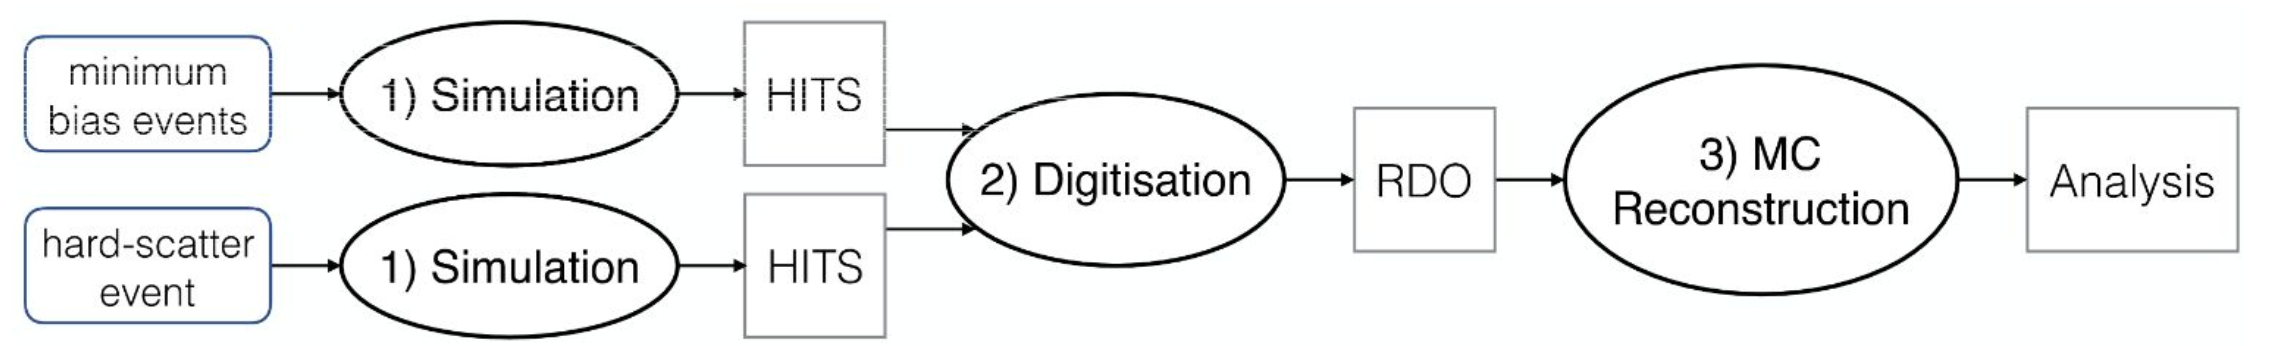
\includegraphics[width=0.9\textwidth]{Chapter2/simulation.png}
	\centering
	\begin{center}
		\caption{The full procedure of the ATLAS simulation}
		\label{Fig:simulation}            
	\end{center}
\end{figure}.

